% Created by tikzDevice version 0.12.3 on 2020-05-24 19:40:37
% !TEX encoding = UTF-8 Unicode
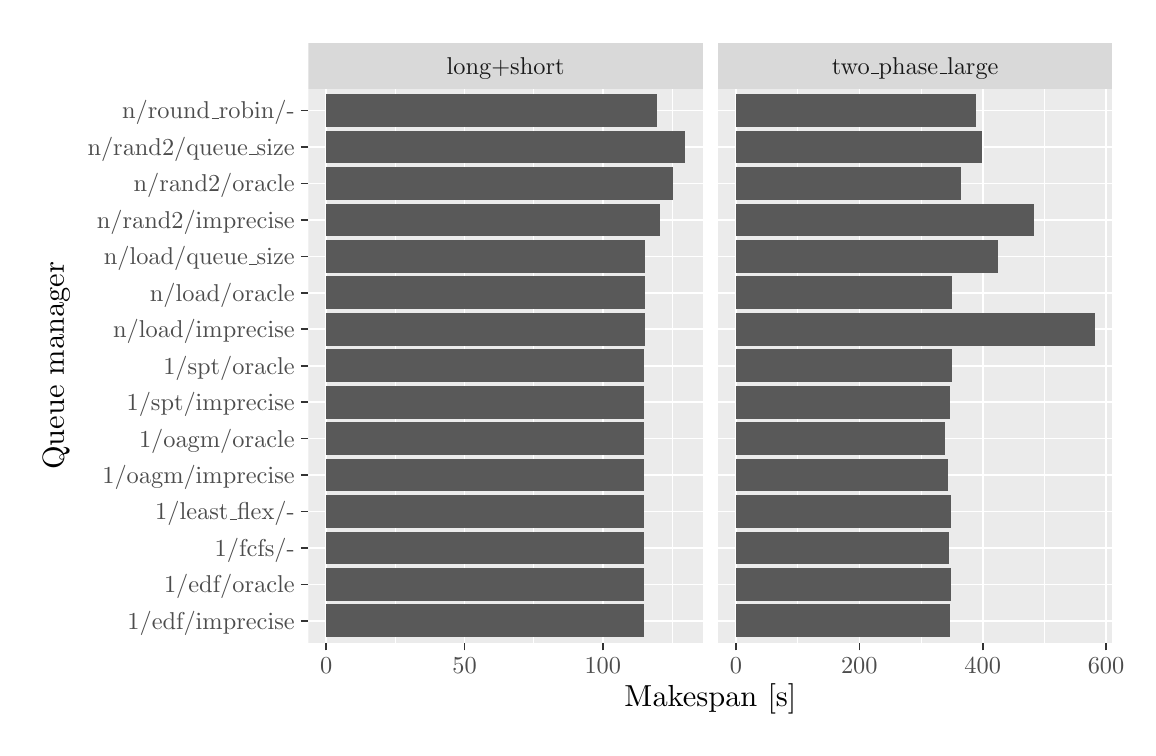
\begin{tikzpicture}[x=1pt,y=1pt]
\definecolor{fillColor}{RGB}{255,255,255}
\path[use as bounding box,fill=fillColor,fill opacity=0.00] (0,0) rectangle (397.48,252.94);
\begin{scope}
\path[clip] (  0.00,  0.00) rectangle (397.48,252.94);
\definecolor{drawColor}{RGB}{255,255,255}
\definecolor{fillColor}{RGB}{255,255,255}

\path[draw=drawColor,line width= 0.6pt,line join=round,line cap=round,fill=fillColor] (  0.00,  0.00) rectangle (397.48,252.94);
\end{scope}
\begin{scope}
\path[clip] (101.44, 30.69) rectangle (243.96,230.87);
\definecolor{fillColor}{gray}{0.92}

\path[fill=fillColor] (101.44, 30.69) rectangle (243.96,230.87);
\definecolor{drawColor}{RGB}{255,255,255}

\path[draw=drawColor,line width= 0.3pt,line join=round] (132.89, 30.69) --
	(132.89,230.87);

\path[draw=drawColor,line width= 0.3pt,line join=round] (182.85, 30.69) --
	(182.85,230.87);

\path[draw=drawColor,line width= 0.3pt,line join=round] (232.81, 30.69) --
	(232.81,230.87);

\path[draw=drawColor,line width= 0.6pt,line join=round] (101.44, 38.59) --
	(243.96, 38.59);

\path[draw=drawColor,line width= 0.6pt,line join=round] (101.44, 51.76) --
	(243.96, 51.76);

\path[draw=drawColor,line width= 0.6pt,line join=round] (101.44, 64.93) --
	(243.96, 64.93);

\path[draw=drawColor,line width= 0.6pt,line join=round] (101.44, 78.10) --
	(243.96, 78.10);

\path[draw=drawColor,line width= 0.6pt,line join=round] (101.44, 91.27) --
	(243.96, 91.27);

\path[draw=drawColor,line width= 0.6pt,line join=round] (101.44,104.44) --
	(243.96,104.44);

\path[draw=drawColor,line width= 0.6pt,line join=round] (101.44,117.61) --
	(243.96,117.61);

\path[draw=drawColor,line width= 0.6pt,line join=round] (101.44,130.78) --
	(243.96,130.78);

\path[draw=drawColor,line width= 0.6pt,line join=round] (101.44,143.95) --
	(243.96,143.95);

\path[draw=drawColor,line width= 0.6pt,line join=round] (101.44,157.12) --
	(243.96,157.12);

\path[draw=drawColor,line width= 0.6pt,line join=round] (101.44,170.29) --
	(243.96,170.29);

\path[draw=drawColor,line width= 0.6pt,line join=round] (101.44,183.46) --
	(243.96,183.46);

\path[draw=drawColor,line width= 0.6pt,line join=round] (101.44,196.63) --
	(243.96,196.63);

\path[draw=drawColor,line width= 0.6pt,line join=round] (101.44,209.80) --
	(243.96,209.80);

\path[draw=drawColor,line width= 0.6pt,line join=round] (101.44,222.97) --
	(243.96,222.97);

\path[draw=drawColor,line width= 0.6pt,line join=round] (107.91, 30.69) --
	(107.91,230.87);

\path[draw=drawColor,line width= 0.6pt,line join=round] (157.87, 30.69) --
	(157.87,230.87);

\path[draw=drawColor,line width= 0.6pt,line join=round] (207.83, 30.69) --
	(207.83,230.87);
\definecolor{fillColor}{gray}{0.35}

\path[fill=fillColor] (107.91, 32.66) rectangle (222.75, 44.51);

\path[fill=fillColor] (107.91, 45.83) rectangle (222.75, 57.68);

\path[fill=fillColor] (107.91, 59.00) rectangle (222.75, 70.86);

\path[fill=fillColor] (107.91, 72.17) rectangle (222.75, 84.03);

\path[fill=fillColor] (107.91, 85.34) rectangle (222.75, 97.20);

\path[fill=fillColor] (107.91, 98.51) rectangle (222.75,110.37);

\path[fill=fillColor] (107.91,111.68) rectangle (222.75,123.54);

\path[fill=fillColor] (107.91,124.85) rectangle (222.75,136.71);

\path[fill=fillColor] (107.91,138.02) rectangle (223.03,149.88);

\path[fill=fillColor] (107.91,151.19) rectangle (223.03,163.05);

\path[fill=fillColor] (107.91,164.36) rectangle (223.03,176.22);

\path[fill=fillColor] (107.91,177.53) rectangle (228.39,189.39);

\path[fill=fillColor] (107.91,190.70) rectangle (233.21,202.56);

\path[fill=fillColor] (107.91,203.87) rectangle (237.48,215.73);

\path[fill=fillColor] (107.91,217.04) rectangle (227.39,228.90);
\end{scope}
\begin{scope}
\path[clip] (249.46, 30.69) rectangle (391.98,230.87);
\definecolor{fillColor}{gray}{0.92}

\path[fill=fillColor] (249.46, 30.69) rectangle (391.98,230.87);
\definecolor{drawColor}{RGB}{255,255,255}

\path[draw=drawColor,line width= 0.3pt,line join=round] (278.23, 30.69) --
	(278.23,230.87);

\path[draw=drawColor,line width= 0.3pt,line join=round] (322.81, 30.69) --
	(322.81,230.87);

\path[draw=drawColor,line width= 0.3pt,line join=round] (367.39, 30.69) --
	(367.39,230.87);

\path[draw=drawColor,line width= 0.6pt,line join=round] (249.46, 38.59) --
	(391.98, 38.59);

\path[draw=drawColor,line width= 0.6pt,line join=round] (249.46, 51.76) --
	(391.98, 51.76);

\path[draw=drawColor,line width= 0.6pt,line join=round] (249.46, 64.93) --
	(391.98, 64.93);

\path[draw=drawColor,line width= 0.6pt,line join=round] (249.46, 78.10) --
	(391.98, 78.10);

\path[draw=drawColor,line width= 0.6pt,line join=round] (249.46, 91.27) --
	(391.98, 91.27);

\path[draw=drawColor,line width= 0.6pt,line join=round] (249.46,104.44) --
	(391.98,104.44);

\path[draw=drawColor,line width= 0.6pt,line join=round] (249.46,117.61) --
	(391.98,117.61);

\path[draw=drawColor,line width= 0.6pt,line join=round] (249.46,130.78) --
	(391.98,130.78);

\path[draw=drawColor,line width= 0.6pt,line join=round] (249.46,143.95) --
	(391.98,143.95);

\path[draw=drawColor,line width= 0.6pt,line join=round] (249.46,157.12) --
	(391.98,157.12);

\path[draw=drawColor,line width= 0.6pt,line join=round] (249.46,170.29) --
	(391.98,170.29);

\path[draw=drawColor,line width= 0.6pt,line join=round] (249.46,183.46) --
	(391.98,183.46);

\path[draw=drawColor,line width= 0.6pt,line join=round] (249.46,196.63) --
	(391.98,196.63);

\path[draw=drawColor,line width= 0.6pt,line join=round] (249.46,209.80) --
	(391.98,209.80);

\path[draw=drawColor,line width= 0.6pt,line join=round] (249.46,222.97) --
	(391.98,222.97);

\path[draw=drawColor,line width= 0.6pt,line join=round] (255.94, 30.69) --
	(255.94,230.87);

\path[draw=drawColor,line width= 0.6pt,line join=round] (300.52, 30.69) --
	(300.52,230.87);

\path[draw=drawColor,line width= 0.6pt,line join=round] (345.10, 30.69) --
	(345.10,230.87);

\path[draw=drawColor,line width= 0.6pt,line join=round] (389.68, 30.69) --
	(389.68,230.87);
\definecolor{fillColor}{gray}{0.35}

\path[fill=fillColor] (255.94, 32.66) rectangle (333.37, 44.51);

\path[fill=fillColor] (255.94, 45.83) rectangle (333.81, 57.68);

\path[fill=fillColor] (255.94, 59.00) rectangle (332.99, 70.86);

\path[fill=fillColor] (255.94, 72.17) rectangle (333.55, 84.03);

\path[fill=fillColor] (255.94, 85.34) rectangle (332.53, 97.20);

\path[fill=fillColor] (255.94, 98.51) rectangle (331.30,110.37);

\path[fill=fillColor] (255.94,111.68) rectangle (333.19,123.54);

\path[fill=fillColor] (255.94,124.85) rectangle (334.03,136.71);

\path[fill=fillColor] (255.94,138.02) rectangle (385.51,149.88);

\path[fill=fillColor] (255.94,151.19) rectangle (333.98,163.05);

\path[fill=fillColor] (255.94,164.36) rectangle (350.66,176.22);

\path[fill=fillColor] (255.94,177.53) rectangle (363.47,189.39);

\path[fill=fillColor] (255.94,190.70) rectangle (337.13,202.56);

\path[fill=fillColor] (255.94,203.87) rectangle (344.93,215.73);

\path[fill=fillColor] (255.94,217.04) rectangle (342.83,228.90);
\end{scope}
\begin{scope}
\path[clip] (101.44,230.87) rectangle (243.96,247.44);
\definecolor{fillColor}{gray}{0.85}

\path[fill=fillColor] (101.44,230.87) rectangle (243.96,247.44);
\definecolor{drawColor}{gray}{0.10}

\node[text=drawColor,anchor=base,inner sep=0pt, outer sep=0pt, scale=  0.88] at (172.70,236.13) {long+short};
\end{scope}
\begin{scope}
\path[clip] (249.46,230.87) rectangle (391.98,247.44);
\definecolor{fillColor}{gray}{0.85}

\path[fill=fillColor] (249.46,230.87) rectangle (391.98,247.44);
\definecolor{drawColor}{gray}{0.10}

\node[text=drawColor,anchor=base,inner sep=0pt, outer sep=0pt, scale=  0.88] at (320.72,236.13) {two\_phase\_large};
\end{scope}
\begin{scope}
\path[clip] (  0.00,  0.00) rectangle (397.48,252.94);
\definecolor{drawColor}{gray}{0.20}

\path[draw=drawColor,line width= 0.6pt,line join=round] (107.91, 27.94) --
	(107.91, 30.69);

\path[draw=drawColor,line width= 0.6pt,line join=round] (157.87, 27.94) --
	(157.87, 30.69);

\path[draw=drawColor,line width= 0.6pt,line join=round] (207.83, 27.94) --
	(207.83, 30.69);
\end{scope}
\begin{scope}
\path[clip] (  0.00,  0.00) rectangle (397.48,252.94);
\definecolor{drawColor}{gray}{0.30}

\node[text=drawColor,anchor=base,inner sep=0pt, outer sep=0pt, scale=  0.88] at (107.91, 19.68) {0};

\node[text=drawColor,anchor=base,inner sep=0pt, outer sep=0pt, scale=  0.88] at (157.87, 19.68) {50};

\node[text=drawColor,anchor=base,inner sep=0pt, outer sep=0pt, scale=  0.88] at (207.83, 19.68) {100};
\end{scope}
\begin{scope}
\path[clip] (  0.00,  0.00) rectangle (397.48,252.94);
\definecolor{drawColor}{gray}{0.20}

\path[draw=drawColor,line width= 0.6pt,line join=round] (255.94, 27.94) --
	(255.94, 30.69);

\path[draw=drawColor,line width= 0.6pt,line join=round] (300.52, 27.94) --
	(300.52, 30.69);

\path[draw=drawColor,line width= 0.6pt,line join=round] (345.10, 27.94) --
	(345.10, 30.69);

\path[draw=drawColor,line width= 0.6pt,line join=round] (389.68, 27.94) --
	(389.68, 30.69);
\end{scope}
\begin{scope}
\path[clip] (  0.00,  0.00) rectangle (397.48,252.94);
\definecolor{drawColor}{gray}{0.30}

\node[text=drawColor,anchor=base,inner sep=0pt, outer sep=0pt, scale=  0.88] at (255.94, 19.68) {0};

\node[text=drawColor,anchor=base,inner sep=0pt, outer sep=0pt, scale=  0.88] at (300.52, 19.68) {200};

\node[text=drawColor,anchor=base,inner sep=0pt, outer sep=0pt, scale=  0.88] at (345.10, 19.68) {400};

\node[text=drawColor,anchor=base,inner sep=0pt, outer sep=0pt, scale=  0.88] at (389.68, 19.68) {600};
\end{scope}
\begin{scope}
\path[clip] (  0.00,  0.00) rectangle (397.48,252.94);
\definecolor{drawColor}{gray}{0.30}

\node[text=drawColor,anchor=base east,inner sep=0pt, outer sep=0pt, scale=  0.88] at ( 96.49, 35.56) {1/edf/imprecise};

\node[text=drawColor,anchor=base east,inner sep=0pt, outer sep=0pt, scale=  0.88] at ( 96.49, 48.73) {1/edf/oracle};

\node[text=drawColor,anchor=base east,inner sep=0pt, outer sep=0pt, scale=  0.88] at ( 96.49, 61.90) {1/fcfs/-};

\node[text=drawColor,anchor=base east,inner sep=0pt, outer sep=0pt, scale=  0.88] at ( 96.49, 75.07) {1/least\_flex/-};

\node[text=drawColor,anchor=base east,inner sep=0pt, outer sep=0pt, scale=  0.88] at ( 96.49, 88.24) {1/oagm/imprecise};

\node[text=drawColor,anchor=base east,inner sep=0pt, outer sep=0pt, scale=  0.88] at ( 96.49,101.41) {1/oagm/oracle};

\node[text=drawColor,anchor=base east,inner sep=0pt, outer sep=0pt, scale=  0.88] at ( 96.49,114.58) {1/spt/imprecise};

\node[text=drawColor,anchor=base east,inner sep=0pt, outer sep=0pt, scale=  0.88] at ( 96.49,127.75) {1/spt/oracle};

\node[text=drawColor,anchor=base east,inner sep=0pt, outer sep=0pt, scale=  0.88] at ( 96.49,140.92) {n/load/imprecise};

\node[text=drawColor,anchor=base east,inner sep=0pt, outer sep=0pt, scale=  0.88] at ( 96.49,154.09) {n/load/oracle};

\node[text=drawColor,anchor=base east,inner sep=0pt, outer sep=0pt, scale=  0.88] at ( 96.49,167.26) {n/load/queue\_size};

\node[text=drawColor,anchor=base east,inner sep=0pt, outer sep=0pt, scale=  0.88] at ( 96.49,180.43) {n/rand2/imprecise};

\node[text=drawColor,anchor=base east,inner sep=0pt, outer sep=0pt, scale=  0.88] at ( 96.49,193.60) {n/rand2/oracle};

\node[text=drawColor,anchor=base east,inner sep=0pt, outer sep=0pt, scale=  0.88] at ( 96.49,206.77) {n/rand2/queue\_size};

\node[text=drawColor,anchor=base east,inner sep=0pt, outer sep=0pt, scale=  0.88] at ( 96.49,219.94) {n/round\_robin/-};
\end{scope}
\begin{scope}
\path[clip] (  0.00,  0.00) rectangle (397.48,252.94);
\definecolor{drawColor}{gray}{0.20}

\path[draw=drawColor,line width= 0.6pt,line join=round] ( 98.69, 38.59) --
	(101.44, 38.59);

\path[draw=drawColor,line width= 0.6pt,line join=round] ( 98.69, 51.76) --
	(101.44, 51.76);

\path[draw=drawColor,line width= 0.6pt,line join=round] ( 98.69, 64.93) --
	(101.44, 64.93);

\path[draw=drawColor,line width= 0.6pt,line join=round] ( 98.69, 78.10) --
	(101.44, 78.10);

\path[draw=drawColor,line width= 0.6pt,line join=round] ( 98.69, 91.27) --
	(101.44, 91.27);

\path[draw=drawColor,line width= 0.6pt,line join=round] ( 98.69,104.44) --
	(101.44,104.44);

\path[draw=drawColor,line width= 0.6pt,line join=round] ( 98.69,117.61) --
	(101.44,117.61);

\path[draw=drawColor,line width= 0.6pt,line join=round] ( 98.69,130.78) --
	(101.44,130.78);

\path[draw=drawColor,line width= 0.6pt,line join=round] ( 98.69,143.95) --
	(101.44,143.95);

\path[draw=drawColor,line width= 0.6pt,line join=round] ( 98.69,157.12) --
	(101.44,157.12);

\path[draw=drawColor,line width= 0.6pt,line join=round] ( 98.69,170.29) --
	(101.44,170.29);

\path[draw=drawColor,line width= 0.6pt,line join=round] ( 98.69,183.46) --
	(101.44,183.46);

\path[draw=drawColor,line width= 0.6pt,line join=round] ( 98.69,196.63) --
	(101.44,196.63);

\path[draw=drawColor,line width= 0.6pt,line join=round] ( 98.69,209.80) --
	(101.44,209.80);

\path[draw=drawColor,line width= 0.6pt,line join=round] ( 98.69,222.97) --
	(101.44,222.97);
\end{scope}
\begin{scope}
\path[clip] (  0.00,  0.00) rectangle (397.48,252.94);
\definecolor{drawColor}{RGB}{0,0,0}

\node[text=drawColor,anchor=base,inner sep=0pt, outer sep=0pt, scale=  1.10] at (246.71,  7.64) {Makespan [s]};
\end{scope}
\begin{scope}
\path[clip] (  0.00,  0.00) rectangle (397.48,252.94);
\definecolor{drawColor}{RGB}{0,0,0}

\node[text=drawColor,rotate= 90.00,anchor=base,inner sep=0pt, outer sep=0pt, scale=  1.10] at ( 13.08,130.78) {Queue manager};
\end{scope}
\end{tikzpicture}
